\newpage
\section{Begriffe}

% ------------------------------------------------------------------------------
\subsection{Definition}

Formal gesehen besteht eine Gleichung aus zwei Termen, die mit einem Gleichheitszeichen verbunden werden:
\[
  \square = \square
\]

% ------------------------------------------------------------------------------
\subsection{Geschichte}

Das Gleichheitszeichen, welches heute verwendet wird, wurde zum ersten Mal vom walisischen Mediziner und Mathematiker Robert Recorde um 1557 verwendet. Die Gleichung $14x+15=71$ hatte er in seinem Buch für Arithmetik so geschrieben:
\begin{center}
  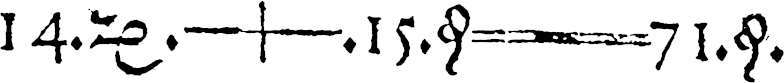
\includegraphics[width=0.4\textwidth]{Erste Gleichung.png}
\end{center}

% ------------------------------------------------------------------------------
\subsection{Aussagen}

In der Mathematik ist eine \textbf{Aussage} eine Behauptung, die entweder \textbf{wahr} oder \textbf{falsch} ist.
\begin{example}
  \textbf{Beispiele:}
  \begin{itemize}[noitemsep]
    \item «Heute scheint die Sonne.»
    \item «Die Wurzel von 25 ist 3.»
    \item «Ich heisse Otto.»
  \end{itemize}
\end{example}
In der Formelsprache der Mathematik werden Aussagen als \textbf{Gleichungen} geschrieben, welche \textbf{keine Variablen} enthalten.
\begin{example}
  \textbf{Beispiele:}
  \begin{itemize}[noitemsep]
    \item Die Aussage $\sqrt{25} = 3$ ist falsch.
    \item Die Aussage $1+1 = 2$ ist wahr.
    \item Die Aussage $1+2 = 4$ ist falsch.
  \end{itemize}
\end{example}
In der Mathematik sind normalerweise nur \textbf{wahre} Aussagen interessant. Falsche Gleichungen können durch die Verwendung des Ungleichheitszeichens $\ne$ in eine wahren Aussage verwandelt werden.
\begin{example}
  \textbf{Beispiele:}
  \begin{itemize}[noitemsep]
    \item Die Aussage $\sqrt{25} \ne 3$ ist wahr.
    \item Die Aussage $1+1 = 2$ ist wahr.
    \item Die Aussage $1+2 \ne 4$ ist wahr.
  \end{itemize}
\end{example}

% ------------------------------------------------------------------------------
\subsection{Aussageformen}

Eine \textbf{Aussageform} ist eine Aussage, welche eine Lücke enthält. Ob die Aussage wahr oder falsch ist, hängt davon ab, was in die Lücke gesetzt wird.
\begin{example}
  \textbf{Beispiele:}
  \begin{itemize}[noitemsep]
    \item «Am \underline{\hspace{1cm}} scheint die Sonne.»
    \item «Die Wurzel von \underline{\hspace{1cm}} ist 3.»
    \item «Ich heisse \underline{\hspace{1cm}}.»
  \end{itemize}
\end{example}
In der Formelsprache der Mathematik werden Aussageformen als \textbf{Gleichungen} geschrieben, welche mindestens eine Variable enthalten. Ob diese wahr oder falsch sind, kann eigentlich erst beurteilt werden, wenn bestimmte Werte für die Variablen eingesetzt werden.
\begin{example}
  \textbf{Beispiel:} $\sqrt{x} = 3$
\end{example}
Wenn in einer Gleichung jede Variable durch eine Zahl ersetzt wird, entsteht eine Aussage, welche entweder wahr oder falsch ist:
\begin{example}
  \textbf{Beispiele:} Die Aussage $\sqrt{16} = 3$ ist falsch. Die Aussage $\sqrt{9} = 3$ ist wahr.
\end{example}
Es gibt aber auch Aussageformen, also Gleichungen mit Variablen, deren Wahrheitsgehalt für alle möglichen Werte der Variablen gleich ist.
\begin{example}
  \textbf{Beispiele:}
  \begin{itemize}[noitemsep]
    \item Die Gleichung $(a+b)^2= a^2+2ab+b^2$ ist für alle Werte $a,b\in\mathbb{R}$ wahr.
    \item Die Gleichung $x=x+1$ ist für alle Werte $x\in\mathbb{R}$ falsch.
  \end{itemize}
\end{example}

% ------------------------------------------------------------------------------
\subsection{Definitionsmenge}

Bei einer Aussageform müssen wir festlegen, welche Werte wir überhaupt in die Lücken einsetzen können, um eine sinnvolle Aussage zu erhalten. So macht die Aussage «Die Wurzel von Otto ist 3.» keinen Sinn.
\begin{example}
  \begin{itemize}[noitemsep]
    \item «Am \underline{\hspace{1cm}} scheint die Sonne.» $\rightarrow$ Setze einen Tag ein.
    \item «Die Wurzel von \underline{\hspace{1cm}} ist 3.» $\rightarrow$ Setze eine reelle Zahl ein.
    \item «Ich heisse \underline{\hspace{1cm}}.» $\rightarrow$ Setze einen Vornamen ein.
  \end{itemize}
\end{example}
Auch bei Gleichungen mit Variablen muss festgelegt werden, welche Zahlen überhaupt für die Variable eingesetzt werden dürfen. Wie bei den Termen heisst die Menge aller erlaubten Zahlen für eine Variable $x$ die \textbf{Definitionsmenge} von $x$ und wird mit $\mathbb{D}_{x}$ bezeichnet.
\begin{example}
  \textbf{Beispiele:}
  $\sqrt{x} = 3 \qquad\Rightarrow\qquad \mathbb{D}_{x} = \mathbb{R}_{0}^{+} \qquad\qquad
    \frac{1}{z+1} = \frac{1}{2} \qquad\Rightarrow\qquad \mathbb{D}_{z} = \mathbb{R}\setminus\{-1\}$
\end{example}

% ------------------------------------------------------------------------------
\subsection{Arten von Gleichungen}

\subsubsection{Identitäten}

Identitäten sind Gleichungen, welche immer wahr sind, egal welche Zahlen aus der Definitionsmengen für die Variablen eingesetzt werden. Identitäten können bewiesen werden, indem die linke Seite der Gleichung mit Hilfe von bekannten Regeln in die rechte Seite umgeformt wird.
\begin{example}
  \textbf{Beispiele:} Die folgenen Gleichungen sind Identitäten:
  \begin{itemize}
    \item Die erste binomische Formel $(a+b)^2= a^2+2ab+b^2$ für $a,b \in\mathbb{R}$.
    \item Das erste Potenzgesetz $a^k\cdot a^m = a^{k+m}$ für $a \in\mathbb{R}, k,m \in \mathbb{Z}$.
  \end{itemize}
\end{example}
Identitäten sind Hilfsmittel in der Mathematik. Sobald sie bewiesen sind, können wir sie einsetzen, um unsere eigenen Umformungen abzukürzen.

\subsubsection{Definitionen}

Mit einer Definition wird ein neuer Begriff eingeführt. Dabei bezieht sich die Definition auf schon Bekanntes. In der Mathematik und Wissenschaft können Definitionen als Gleichung geschrieben werden.
\begin{example}
  \textbf{Beispiele:} Die Kreiszahl Pi $\pi$ wird als Verhältnis des Umfang $U$ eines Kreises zu seinem Durchmesser $d$ definiert:
  \[
    \pi := \frac{U}{d}
  \]
  In der Physik wird die Arbeit $W$ als die benötigte Kraft $F$ mal der zurückgelegte Weg $s$ definiert:
  \[
    W := F\cdot s
  \]
\end{example}
Dabei wird für den neuen Begriff ein Symbol definiert. Damit klar ersichtlich ist, welches das neu definierte Symbol ist, wird manchmal das Definitions-Gleichheitszeichen $:=$ verwendet. Auf der anderen Seite des Gleichheitszeichen steht ein Term, welcher angibt, wie der neue Wert aus bekannten Werten berechnet wird.

\newpage
\subsubsection{Bestimmungsgleichungen}

Bestimmungsgleichungen sind Aussageformen, also Gleichungen mit mindestens einer Variable, welche nicht notwendigerweise für alle Werte aus der Definitionsmenge eine wahre Aussage ergeben.
\begin{example}
  \textbf{Beispiel:} Die folgende Gleichung wird zu einer wahren Aussage, wenn wir für $x$ der Wert $5$ oder $-5$ eingesetzt wird:
  \[
    x^2 = 25
  \]
\end{example}

% ------------------------------------------------------------------------------
\subsection{Gleichungen Lösen und Lösungsmenge}

Das Bestimmen der Werte aus der Definitionsmenge, für welche eine Gleichung zu einer wahren Aussage wird, wird das \textbf{Lösen der Gleichung} genannt. Die Menge aller Werte, welche die Gleichung zu einer wahren Aussage machen, heisst \textbf{Lösungsmenge} und wird mit dem Zeichen $\mathbb{L}$ abgekürzt.

\begin{example}
  \textbf{Beispiele:} Die Definitionsmenge ist $\mathbb{D} = \mathbb{R}$.
  \begin{align*}
     2x = 10 \qquad&\Rightarrow\qquad \mathbb{L} = \{5\} \\
    x^2 = 25 \qquad&\Rightarrow\qquad \mathbb{L} = \{-5; 5\} \\
    x^4 = -4 \qquad&\Rightarrow\qquad \mathbb{L} = \{\}
  \end{align*}
\end{example}

Um eine Gleichung zu lösen, wird die Gleichung so umgeformt, dass eine Variable \textbf{isoliert} auf einer Seite der Gleichung steht. Das bedeutet, dass die Gleichung in die folgende Form gebracht wird:
\[
  x = \square
\]
wobei $\square$ ein Term ist, der $x$ nicht enthält. Dann kann die Lösung abgelesen werden, indem der Wert des Terms bestimmt wird.
